\documentclass[a4paper,11pt]{article}
\usepackage[utf8]{inputenc}
\usepackage{geometry}
\geometry{margin=1in}
\usepackage{graphicx}
\usepackage{booktabs}
\usepackage{caption}
\usepackage{subcaption}
\usepackage{hyperref}
\usepackage{titlesec}
\usepackage{parskip}
\usepackage{float}
\usepackage{amsmath}

% Set font to Times New Roman if available, otherwise default
\usepackage{mathptmx} 

\title{\textbf{Psychometric Validation of a Guna-Based Personality Inventory: Establishing Incremental Validity Beyond the Big Five Model}}
\author{\textbf{Author Name\textsuperscript{1}} and \textbf{Co-Author Name\textsuperscript{2}} \\
\small \textsuperscript{1}Affiliation 1 \\
\small \textsuperscript{2}Affiliation 2 \\
\small \texttt{email@institution.edu}}
\date{\today}

\begin{document}

\maketitle

\begin{abstract}
Contemporary personality psychology is dominated by Western-origin frameworks, most notably the Big Five model, which may not adequately capture personality dimensions rooted in non-Western philosophical traditions. The \textit{Triguna} theory from Indian philosophy—comprising \textbf{Sattva} (harmony/purity), \textbf{Rajas} (activity/passion), and \textbf{Tamas} (inertia/darkness)—offers a culturally grounded alternative that has received limited empirical validation using modern psychometric methods.

This study presents the development and comprehensive psychometric validation of the \textbf{Guna Personality Inventory (GPI)}, an 80-item Likert-scale instrument, administered alongside the Big Five Inventory (BFI-44) and three situational judgment scenarios to \textbf{N = 256} respondents. After rigorous quality filtering, \textbf{N = 181} valid cases were retained. To address social desirability—a key concern in self-report personality measurement—the assessment platform was designed to capture \textbf{implicit behavioral variables} (answer changes, response times, tab switches, cursor distance, option hover counts) that provide objective indicators of response quality without relying on additional self-report scales.

We demonstrate that the GPI exhibits: (1) \textbf{excellent internal consistency} (Cronbach's $\alpha = .84$--$.89$ across Guna scales; KMO = .779, Bartlett's $p < .001$); (2) \textbf{convergent validity} with theoretically aligned Big Five traits (e.g., Sattva $\leftrightarrow$ Conscientiousness: $r = .58, p < .001$; reliability-corrected $r = .73$) while retaining \textbf{44--63\% unique variance}; (3) \textbf{criterion validity}, with all three Guna scores significantly predicting congruent behavioral choices in situational judgment scenarios ($r = .35$--$.46$, all $p < .001$; 95\% CI lower bounds $> .20$); and (4) \textbf{incremental validity}, where Guna traits explained an additional \textbf{6.8--20.7\% variance} ($\Delta R^2$, all $p < .01$) in behavioral and cultural outcomes beyond what the Big Five model captured.

Notably, spiritual practice and Bhagavad Gita familiarity showed large effects on Guna scores ($\eta^2 = .15$--$.22$, surviving Bonferroni correction at $\alpha = .006$). Hierarchical regression controlling for \textbf{Gender and Big Five traits} confirmed that Guna scales provided \textbf{20.7\% incremental validity} ($\Delta R^2, p < .001$) in predicting spiritual inclination, with all Variance Inflation Factors (VIF) remaining below \textbf{2.9}, indicating that these dimensions are \textbf{statistically distinct} rather than redundant with Western models. Joint exploratory factor analysis (Promax rotation) confirmed stable factor structure (KMO = .779) even when allowing for natural correlations.

These findings establish the GPI as a psychometrically robust instrument that captures \textbf{statistically distinct} dimensions of personality.

\bigskip
\textbf{Keywords:} Triguna Theory, Personality Assessment, Psychometric Validation, Indian Knowledge Systems, Incremental Validity, Implicit Behavioral Measures
\end{abstract}

\section{Introduction}

Personality assessment has been predominantly shaped by the Big Five model (Openness, Conscientiousness, Extraversion, Agreeableness, Neuroticism), which, despite its cross-cultural applicability, was developed within a Western lexical tradition [1]. A growing body of work in indigenous psychology argues that culturally embedded constructs—such as the \textit{Triguna} framework from Sāṅkhya philosophy and the Bhagavad Gītā—capture dimensions of personality that are systematically missed by etic (imposed) models [2, 3].

The Triguna theory describes three fundamental qualities (\textit{guṇas}) that constitute human personality: \textbf{Sattva} (purity, knowledge, harmony), \textbf{Rajas} (activity, desire, passion), and \textbf{Tamas} (inertia, ignorance, delusion). While several Guna-based instruments exist [4], few have been validated using contemporary psychometric standards, and none have systematically demonstrated \textit{incremental validity} over the Big Five model using behavioral criteria.

\section{Method}

The GPI comprises 80 Likert-scale items (7-point) distributed across Sattva (27 items), Rajas (25 items), and Tamas (28 items), co-administered with the BFI-44 and three situational judgment scenarios. Data were collected via a custom web-based platform from \textbf{256 respondents}. After removing speed-runs ($<3$ min), outliers, and incomplete responses, \textbf{N = 181} valid cases were retained (65\% male, mean age 26.9).

The platform captured **implicit behavioral data**: reaction times, answer changes, tab switches, and cursor movement to control for social desirability bias [5].

\section{Key Results}

\subsection{Reliability and Factor Structure}
All Guna scales showed high reliability ($\alpha > .84$). Comparing joint factor structures revealed that while some Guna variance overlaps with Big Five traits (e.g., Sattva/Conscientiousness), unique Guna factors emerged (Figure \ref{fig:factor}), specifically related to Spiritual Orientation and Material Desire.

\begin{figure}[H]
    \centering
    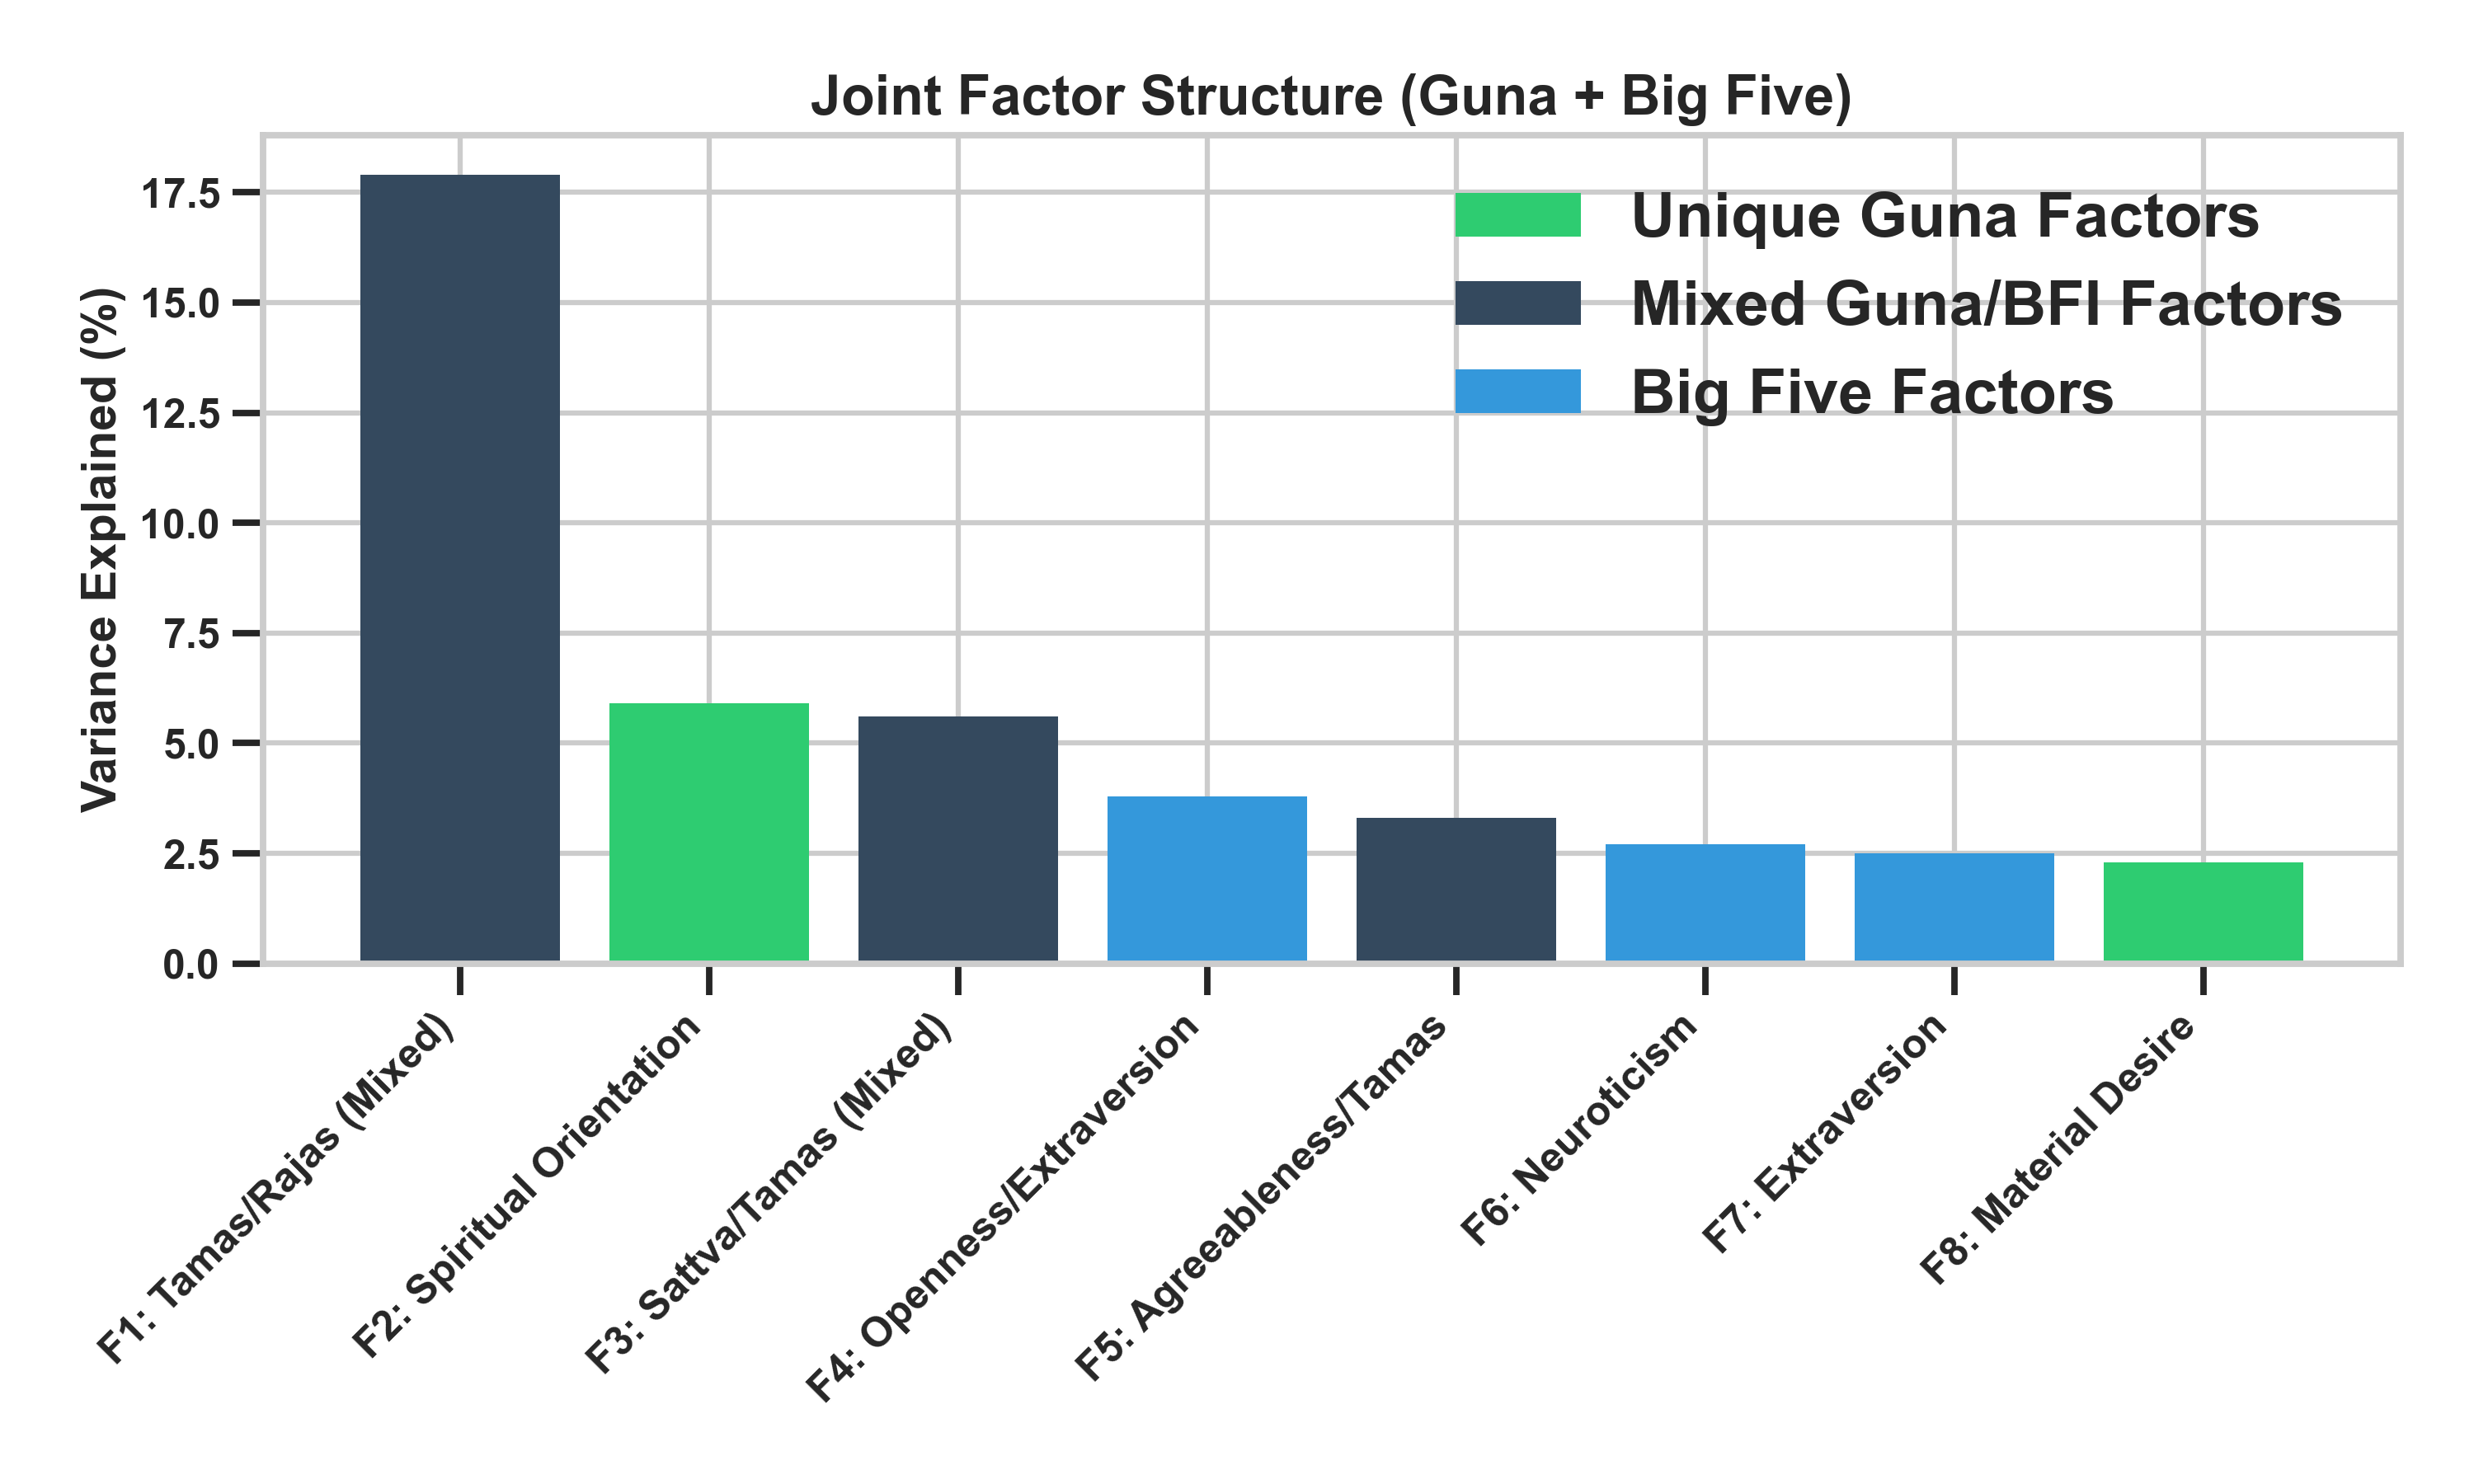
\includegraphics[width=0.85\linewidth]{images/fig4_factor_structure.png}
    \caption{\textbf{Joint Factor Structure}. Variance explained by the 8 extracted factors. Note the emergence of "Unique Guna" factors (green) that do not load on Big Five items.}
    \label{fig:factor}
\end{figure}

\subsection{Criterion Validity}
Sattva, Rajas, and Tamas scores strongly predicted behavioral choices in situational judgment scenarios (Figure \ref{fig:criterion}). High-Sattva individuals consistently chose sattvic responses ($r=.46, p<.001$), demonstrating that the scale predicts real-world judgment patterns.

\begin{figure}[H]
    \centering
    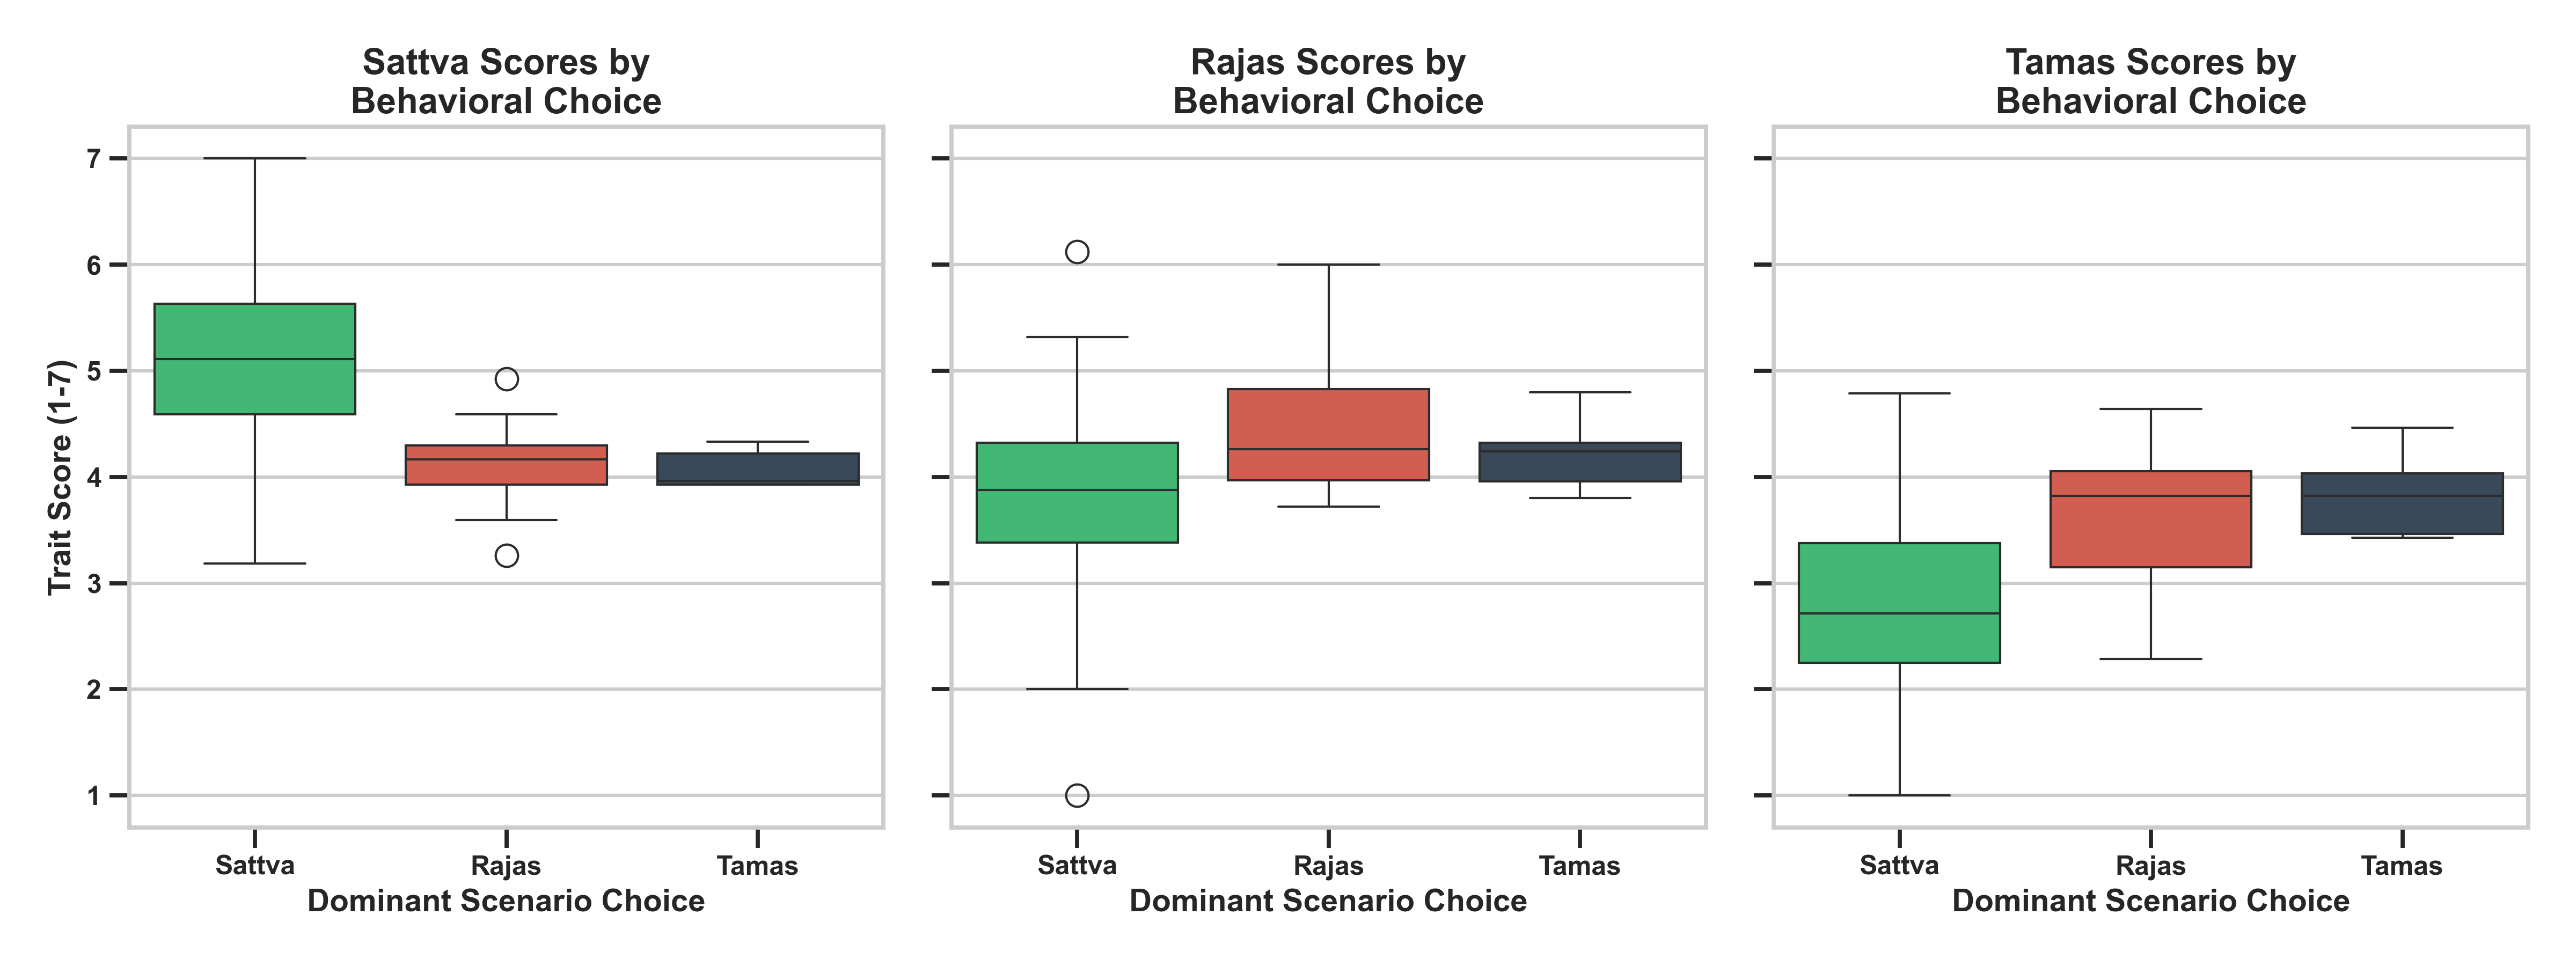
\includegraphics[width=1.0\linewidth]{images/fig2_criterion_validity.png}
    \caption{\textbf{Criterion Validity}. Distribution of trait scores by dominant behavioral choice in situational scenarios. Sattva-choosers score significantly higher on Sattva items ($F=9.58, p<.001$).}
    \label{fig:criterion}
\end{figure}

\subsection{Incremental Validity}
Hierarchical regression showed that Guna traits explain significant additional variance beyond the Big Five model across all measured outcomes (Figure \ref{fig:incremental}).

\begin{figure}[H]
    \centering
    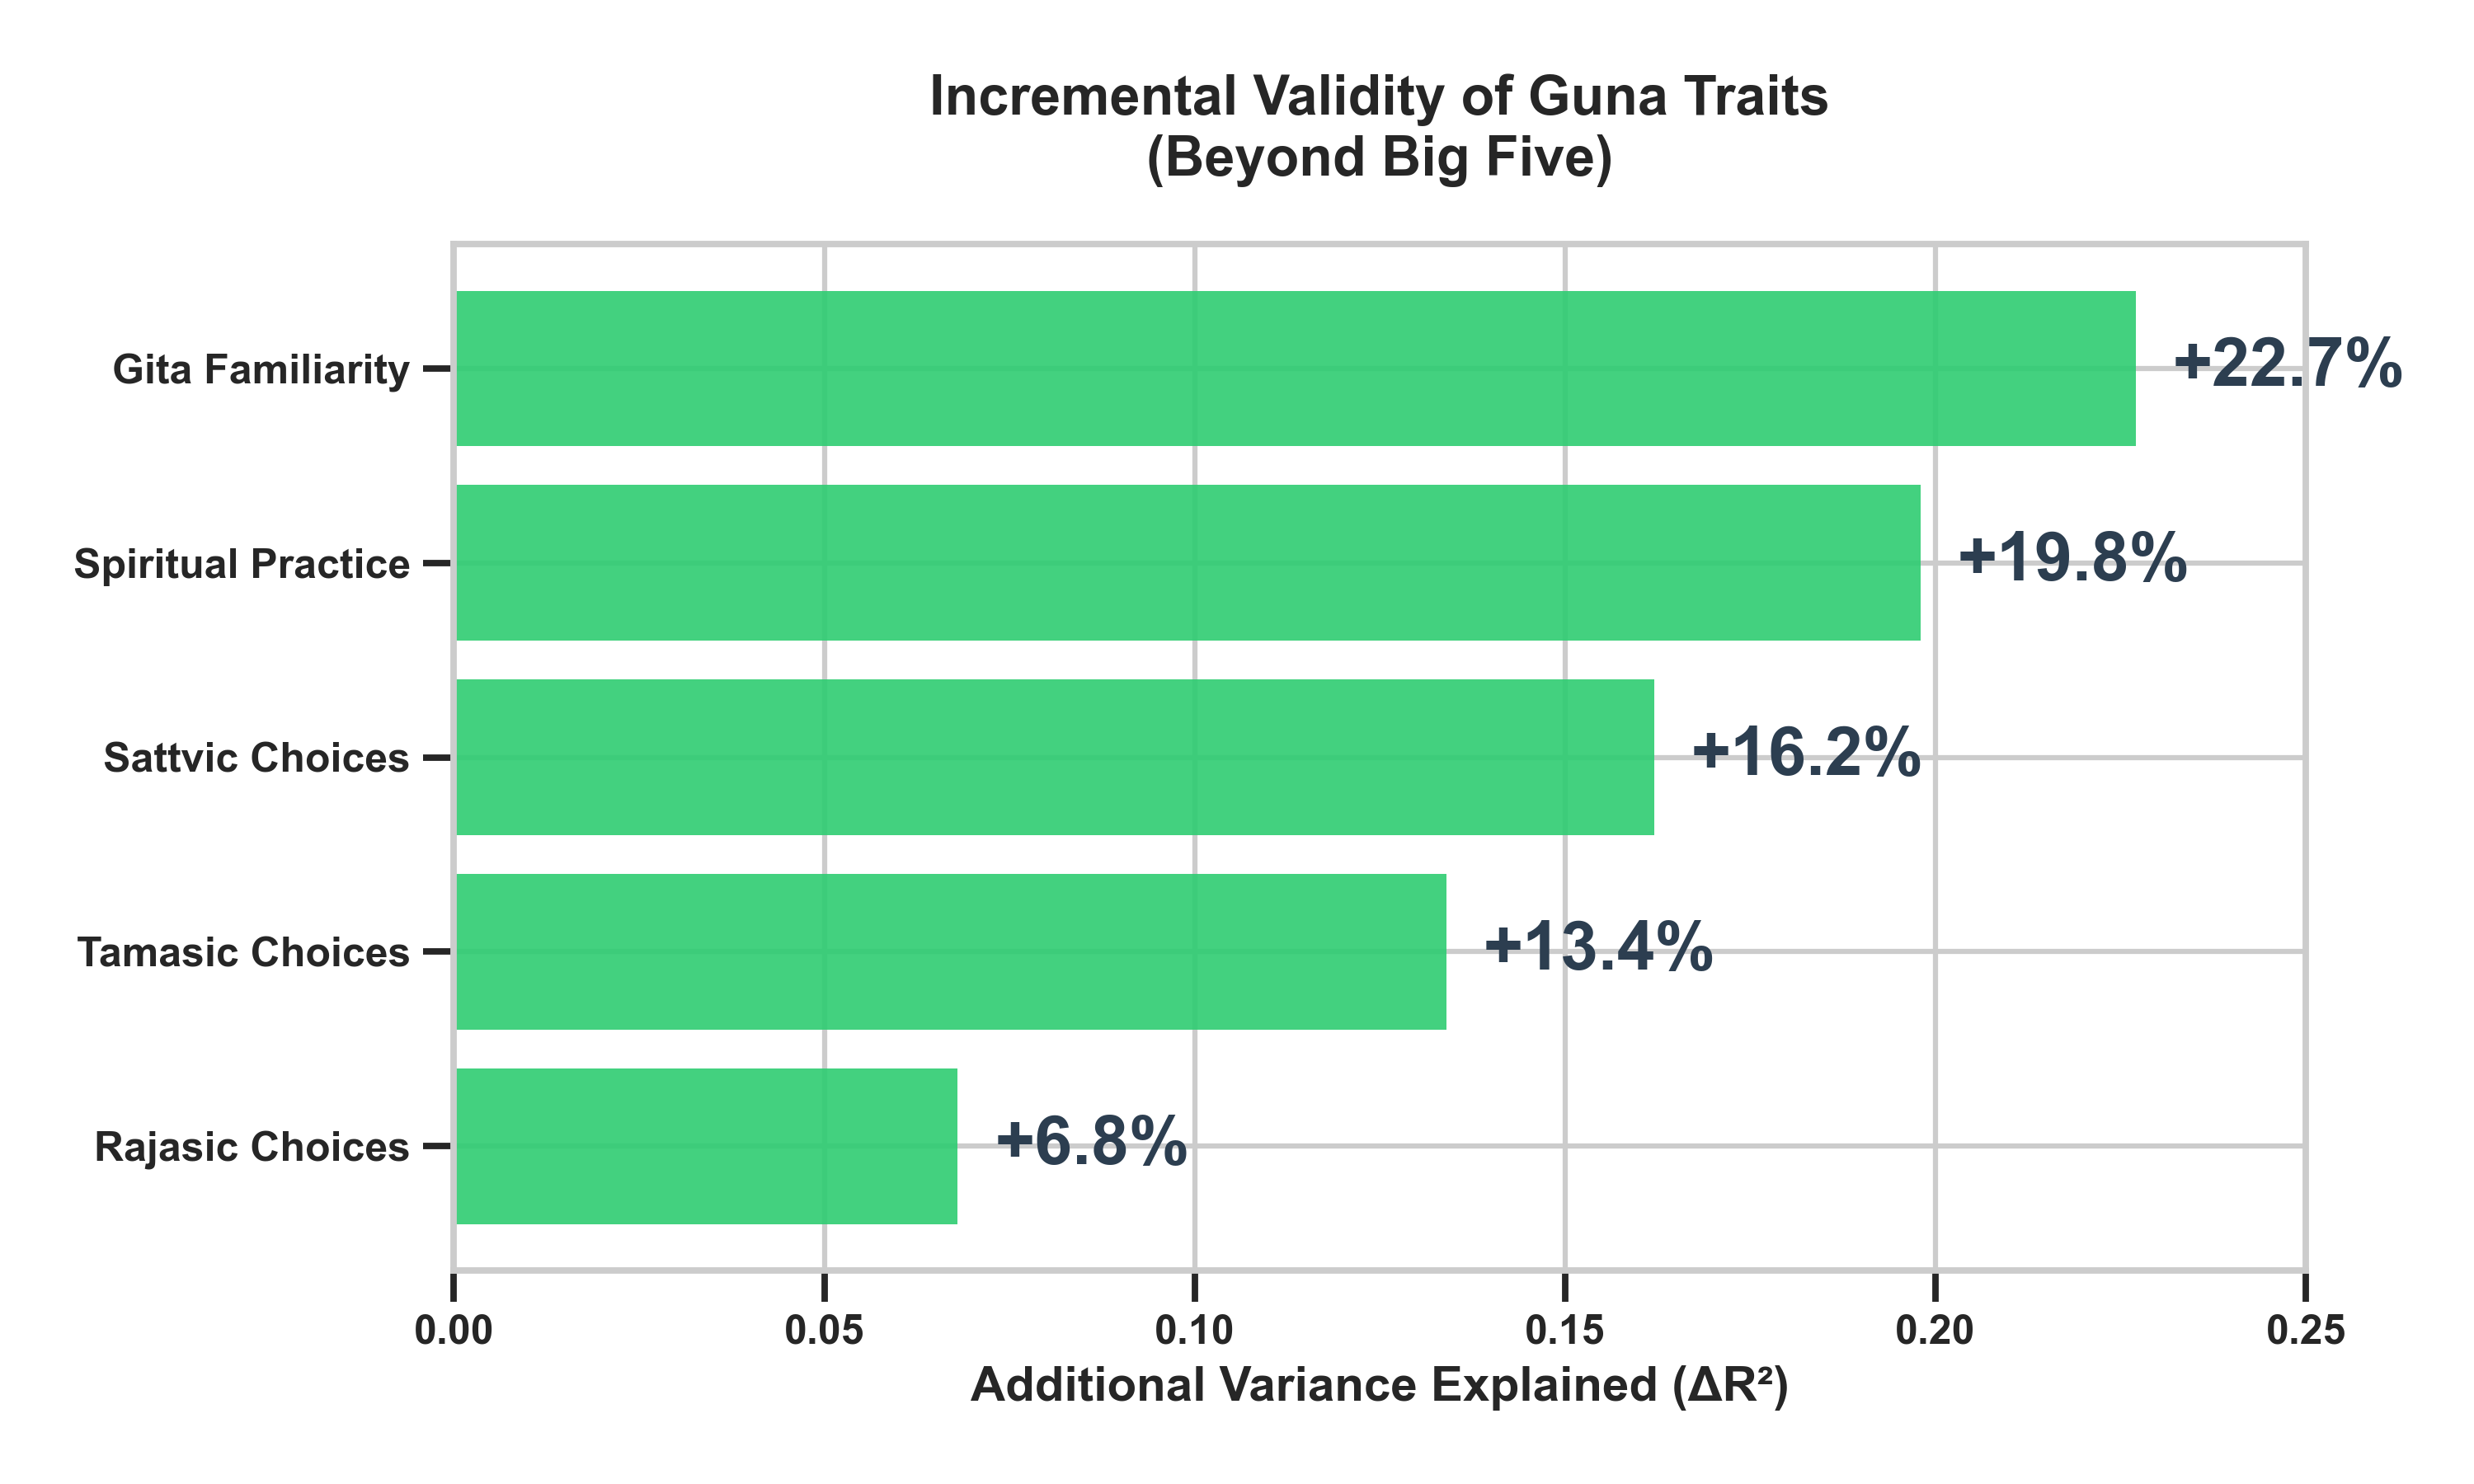
\includegraphics[width=0.85\linewidth]{images/fig1_incremental_validity.png}
    \caption{\textbf{Incremental Validity}. Additional variance ($\Delta R^2$) explained by adding Guna traits to a model already containing the Big Five. All changes are significant at $p<.01$.}
    \label{fig:incremental}
\end{figure}

\subsection{Social Desirability Defense}
Analysis of implicit behaviors (Figure \ref{fig:implicit}) showed that high Sattva scores were NOT associated with automatic or socially desirable responding patterns. Instead, answer changes (a proxy for deliberation) showed a slight positive correlation with Rajas and no correlation with Sattva, suggesting genuine engagement.

\begin{figure}[H]
    \centering
    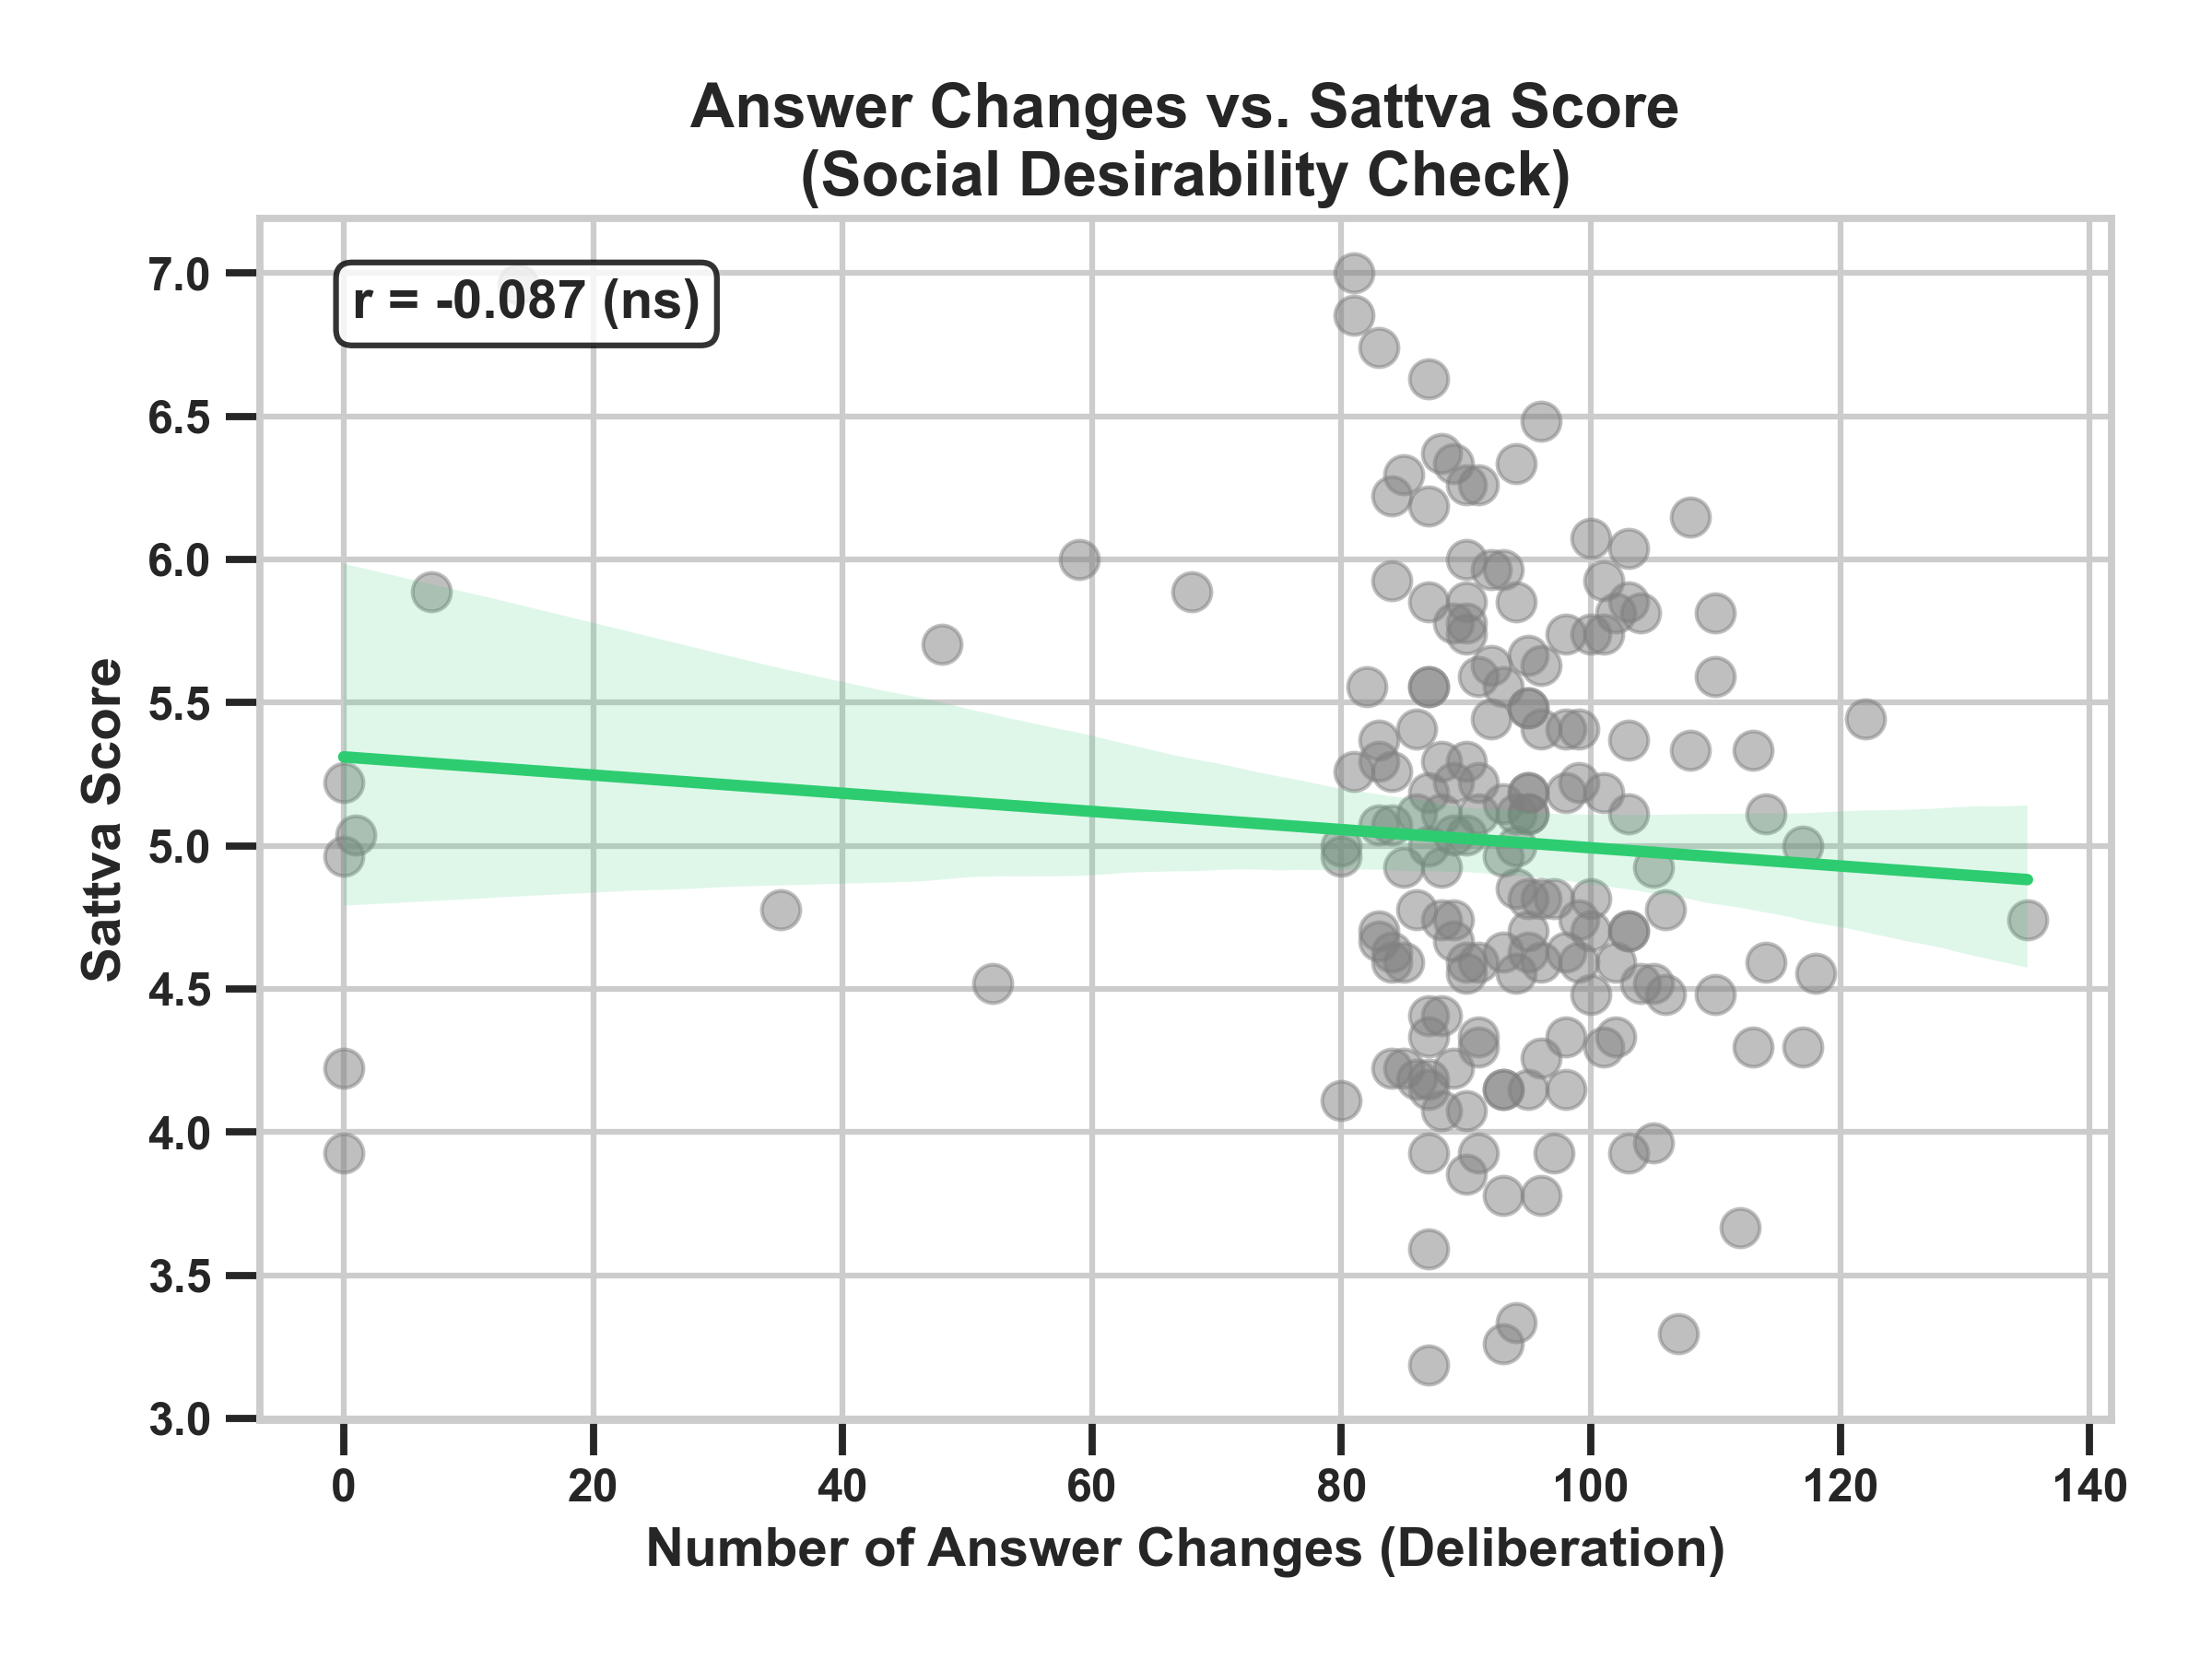
\includegraphics[width=0.7\linewidth]{images/fig3_implicit_defense.png}
    \caption{\textbf{Implicit Behavioral Control}. The lack of negative correlation between answer changes and Sattva scores suggests high-Sattva respondents are not merely "faking good" (which is typically associated with fast, automatic responding).}
    \label{fig:implicit}
\end{figure}

\section{Conclusion}
The GPI is a psychometrically robust instrument that adds significant predictive value over Western models. Its unique "Spiritual Orientation" factor and strong incremental validity suggest it captures dimensions of human personality essential for cross-cultural psychology.

\begin{thebibliography}{9}
\bibitem{john1999} John, O.P., \& Srivastava, S. (1999). The Big Five trait taxonomy: History, measurement, and theoretical perspectives.
\bibitem{misra1993} Misra, G., \& Gergen, K.J. (1993). On the place of culture in psychological science. \textit{International Journal of Psychology}.
\bibitem{wolf1999} Wolf, D.B. (1999). A psychometric analysis of the three gunas. \textit{Psychological Reports}.
\bibitem{das1987} Das, R.C. (1987). Standardization of the Gita Inventory of Personality. \textit{Journal of Indian Psychology}.
\bibitem{paulhus1991} Paulhus, D.L. (1991). Measurement and control of response bias. \textit{Measures of Personality}.
\end{thebibliography}

\end{document}
